\chapter{Firmware}

En aquest capítol es detallarà tot el referent al codi que anirà dintre de la
placa de circuit imprès realitzada en el capítol anterior. Degut que les
connexions entre la placa creada i l'entorn de proves amb la placa \est{Digispark}
i el mòdul \est{GY521} són idèntiques, el \est{firmware} que es crei servirà
per les dues plaques.

Tal i com s'ha dit en l'apartat \ref{subsec:hw_digispark}, es va descobrir
el projecte \est{i2c\_on\_littlewire}, que permet comunicar-se directament amb
dispositius \acro{i2c} des de l'ordinador. En aquest apartat també es destaquen
els motius pel que s'ha descartat aquesta possiblitat, però tot i això cal
mencionar que es va crear un petit codi de C per a demostrar que la comunicació
era possible. Aquest codi es va basar en els exemples disponibles a
\cite{I2cTinyUsb}.

\section{Entorn de treball de desenvolupament}

Per a poder desenvolupar amb comoditat el \est{firmware} del projecte és crucial
facilitar la tasca de provar les modificacions fetes. Per aquest motiu, s'ha
planejat tot un entorn de treball que es detalla en aquest apartat.

\subsection{\est{Bootloader}}
\label{subsec:bootloader}

Hi ha diverses formes de programar el microcontrolador, però la més adequada
per al sistema en qüestió, i tenint present que es voldrà programar el dispositiu
moltes vegades, és utilitzar un \est{bootloader} que identifiqui el dispositiu
com una placa programable durant els primers segons d'operació. Si al cap de
poc temps que el dispositiu no estigui alimentat l'usuari no ha intentat
programar-hi res a través de l'ordinador, s'executarà el programa principal
del microcontrolador.

Aquest \est{bootloader} que s'ha descrit és exactament el que hi ha en la
placa \est{Digispark} per defecte. Com és evident, en un producte definitiu no
interessa posar un \est{bootloader} que retardi el començament del programa
uns segons més, però per a fer proves valdrà la pena aquesta espera.

Programar el \est{Digispark} o una placa equivalent com la d'aquest projecte
utilitzant el \est{bootloader} definit anteriorment és una tasca molt senzilla.
Un cop es disposi del fitxer \fitx{.hex} que es vol programar al
microcontrolador, es pot utilitzar programes com \ord|avrdude| o
\est|micronucleus| per a que, mentre s'estigui executant el bootloader, es 
reprogrami el xip \cite{DigisparkBootloader}.

Per a progrmar la placa amb un sistema basat en Linux s'ha de realitzar una
tasca extra: els permisos. Un usuari administrador podrà programar la placa
sense cap problema, però executar com a \est{root} un programa sempre implica
assumir riscos. Per això el més recomanat és crear una regla \acro{udev}
per al dispositiu en qüestió, fent que sigui accessible per a tots els usuaris.
Es pot consultar un tutorial detallat a \cite{CreateUdevRules}.

\subsection{\est{Makefile}}

Un cop es sap com programar la placa, el següent pas a seguir és crear un
\est{Makefile} per a poder compilar i programar amb una única comanda.
No és la primera ni la segona vegada que s'utilitza l'eina \ord|make| en
aquesta titulació però sí que és la primera vegada que s'utilitza amb una placa
que no sigui un Arduino. Tanmateix, no hi ha gaire diferència, tret de la
part de programar mencionada en l'apartat anterior.

S'ha preparat i documentat el \est{Makefile} com es mereix: s'ha posat un menú
d'ajuda, s'ha posat l'opció per a programar els fusibles del microcontrolador
(aquesta part només s'ha de fer una sola vegada), s'ha posat opcions per a
eliminar tots els fitxers generats i també per a poder debugar el programa.

\section{\acro{V-usb}}

Amb l'entorn de programació preparat, ja es pot començar a crear el
\est{firmware} del projecte. Es començarà per la part més complicada: la
llibreria \acro{v-usb}. Tanmateix, aquesta té molt bona documentació i
tutorials disponibles per internet.

La tasca d'aquest apartat és aconseguir que l'ordinador identifqui la placa
com un acceleròmetre tridimensional. Per a arribar a aquesta meta hi haurà un
seguit de reptes i barreres a superar.

El punt de partida és els codis d'exemples del repositori del projecte
\cite{VusbProjects}.
També hi ha un repositori amb bastants exemples, però la majoria només son
compatibles per a un \acro{AtMega}, i s'haurien d'adaptar de totes formes.

\subsection{Ca\l.libració de l'osci\l.loscopi}

Un dels problemes més grans del microcontrolador que s'està utilitzant és que
l'osci\l.lador intern que disposa no és compatible amb el que demana el
protocol \acro{usb}. Es disposa d'una freqüència de
\SI[round-mode=places,round-precision=1]{16.5}{\mega\hertz} i
\acro{usb2} funciona a
\SI[round-mode=places,round-precision=0]{1}{\kilo\hertz}.

Aquest problema és ben conegut pels desenvolupadors de \acro{v-usb} i en alguns
dels exemples s'explica com ca\l.librar l'osci\l.lador intern per a poder-se
comunicar amb \acro{usb2} basant-se en els intèrvals de temps entre els que es
reb senyal des de l'ordinador. Es recomana consultar aquests codis
\cite{Vusb} si es vol entendre millor aquest apartat.

No utilitzar un rellotge compatible amb el protocol \acro{usb} viola les normes
marcades per la propia entitat \acro{usb-if}. Tanmateix, com s'ha vist en
apartats anteriors, no es pretén certificar com a \acro{usb} el dispositiu
(per altres motius no tècnics), pel que mentre funcioni correctament en la
àmplia majoria de dispositius es considerarà un èxit.

\subsection{Identificadors USB}

Parlant de \acro{usb-if}, en aquest punt del projecte és quan s'ha de decidir
quin \acro{vid-pid} es posa al dispositiu, si més no, durant el temps de
desenvolupament. Tal i com s'ha vist en l'apartat \ref{subsec:usb-if}, hi ha dues
opcions possibles.

Durant el desenvolupament es decidirà utilitzar un parell de codis sense
consensuar-ho amb ningú. Aquesta és la solució més senzilla i ràpida, ja que per
a obtenir identificadors a partir d'entitats mencionades anteriorment es sol
tardar un temps, i acostumen a acceptar únicament projectes acabats o en fase
de proves finals.

Així doncs, s'ha optat per a agafar el \acro{vid-pid}
\texttt{0x16c0}-\texttt{0x09e8}, que és la
parella de codis que els autors de \acro{v-usb} ofereixen per a fer proves
individuals \cite{Vusb}. En altres paraules, \est{ObDev}, el propietari dels
codis, mai assignarà aquests identificadors a un producte que acabi sent
comercialitzat. Va perfecte doncs per a fer proves durant el desenvolupament del
projecte.

\subsection{\est{Watchdog}}

Una altra de les funcionalitats afegides en aquest projecte és el \est{watchdog}.
Es tracta d'un perifèric disponible en la majoria de xips de l'arquitectura
\acro{avr} (entre d'altres) que té per objectiu detectar anomalies durant
l'execució del programa.

Un \est{watchdog} disposa d'un temporitzador que el programa principal ha d'anar
reiniciant cada poc temps. Si passa més d'un llindar de temps sense que el
temporitzador ha sigut reiniciat es considera que el programa principal s'ha
quedat penjat, i el \est{watchdog} actua. Es pot configurar perquè actui de
diferents maneres, però la més senzilla i popular és reiniciant el programa
sencer amb un \est{flag} activat, perquè el mateix programa pugui detectar que
no ha sigut un reinici voluntari, sinó degut a un error previ \cite{Watchdog}.

La llibreria \acro{v-usb} disposa d'exemples on s'utilitza un \est{watchdog}, i
per tant no ha sigut gaire complicació afegir-lo en aquest projecte. És una
protecció adicional per a assegurar-se que el dispositiu sempre funciona
correctament, o com a mínim sense errors greus que no permetin l'execució
normal del programa.

\subsection{Canvi de tipus HID}

Finalment, la tasca més complicada d'implantar aquesta llibreria en el marc
del treball de final de grau és la configuració del nou tipus \acro{hid}:
acceleròmetre tridimensional.

Resulta que els tutorials documenten molt bé com configurar tota la llibreria,
però no és cosa seva explicar com es creen o modifiquen \est{Hid Report Descriptors}.
Tot i que hi ha exemples amb la llibreria que utilitzen la classe \acro{hid},
aquests són per a simular teclats o ratolins. S'ha hagut de buscar molt per a
trobar una mica d'inforamció al respecte.

Tanmateix, després de molt prova i error i anar debugant amb l'ajuda de
\est{wireshark} totes les comunicacions (es recomana configurar \est{wireshark}
d'acord amb aquest tutorial per a rebre paquets \acro{usb}
\cite{InstallWireshark}), s'ha aconseguit
generar un \est{Hid Report Descriptor} que és correctament llegit per l'ordinador.
Una de les referències més importants sobre aquesta part és \cite{VusbProjects}.

\section{I2C}

Un cop solucionada la comunicació entre el microcontrolador i l'ordinador, toca
centrar-se en la comunicació entre el microcontrolador i el sensor. Aquesta, tal
i com s'ha dit en el capítol anterior, es farà mitjançant el protocol \acro{i2c}.
Aquest protocol utilitza dues línies bidireccionals, una per les dades i una per
el rellotge, que es connecten a \SI[round-mode=places,round-precision=0]{0}{\volt}
o es deixen a l'aire (i els \est{pull-ups} la porten a la tensió d'alimentació).

Si bé hi ha moltes llibreries per a la placa Arduino i altres microcontroladors
de l'arquitectura \acro{avr}, totes utilitzen perifèrics específics que, en el
cas de l'\acro{AtTiny85} d'aquest projecte, o estan ja en ús per \acro{v-usb}, o
no existeixen per a aquest xip. Així doncs, s'ha de aprendre el funcionament a
baix nivell del protocol i implementar-lo des de zero.

Per sort, aquest protocol no és molt extens i amb unes 300 línies de codi en C
s'ha pogut implementar el parell de funcions que es necessitava per a dur a
terme el projecte.

El protocol \acro{i2c}, com s'ha dit anteriorment, és molt versàtil i permet 
to\l.lerar dispositius amb diferents tensions d'alimentació, més dispositius
(esclaus, però també mestres) i molta escalabilitat. El mestre és qui inicia
la transmissió (per tant, dos esclaus no poden parlar entre si), però la
direcció del flux de dades pot canviar \cite{I2c}.

El funcionament de \acro{i2c} es pot resumir en poques paraules: el mestre envia
pel canal una adreça de 7 bits per a saber amb quin dispositiu vol comunicar-se.
Aquests 7 bits són l'adreça del dispositiu, disponible als \est{datasheets}. Per
al sensor d'aquest projecte, l'adreça és \texttt{0x68} \cite{MPU6050reg}.
Després d'aquests 7 bits,
s'envia un vuitè bit que dependrà de si es vol enviar dades o rebre dades del
dispositiu.

Un cop rebut el \est{acknowledgement} de l'esclau, comença la transmissió de
dades, que acabarà en funció dels valors de \est{acknowledgement} del mestre, o
si el mestre envia un senyal de stop. Es recomana llegir el \est{dataheet} del
sensor a \cite{mpu6050specs} per a entendre el funcionament de \acro{i2c},
ja que està molt ben explicat.

\subsection{Funcionament del sensor \est{MPU6050}}

Pel cas concret del sensor d'aquest projecte, hi ha un parell de normes extres
a part de les que estableix el protocol \acro{i2c} que serveixen per a comunicar-se
d'una forma fiable amb el sensor.

El sensor \est{MPU6050} defineix en el seu \est{datasheet} un seguit de
registres, que funcionen de la mateixa forma que els perifèrics en \acro{avr}:
no son registres comuns per a guardar dades, sinó que és com si hi hagués una
extensió en els perifèrics del propi microcontrolador. Així doncs, si es llegeix
els registres \texttt{0x42:0x41} es podrà consultar el valor mesurat de temperatura
(sense processar) \cite{MPU6050reg}. També es pot escriure en alguns registres,
per exemple per a activar o ca\l.librar el sensor.

Per a escriure en un registre només cal enviar per \acro{i2c} (és a dir, escriure)
l'adreça del registre i el valor a escriure. Si s'envien més bytes, el sensor
entendrà que s'han d'escriure en els registres posteriors. Pel que fa a la lectura,
s'ha d'enviar l'adreça del registre i tornar a escriure la capçalera \acro{i2c},
però en aquest cas, en mode de lectura. El sensor enviarà els continguts del
registre en qüestió. Si es decideix de seguir llegint (mitjançant un \acro{nack}),
el sensor enviarà el valor del registre posterior \cite{mpu6050specs}.

Finalment, cal destacar que, pel que fa al sensor, poca configuració se li ha de
fer per a rebre dades d'acceleració. Només cal desactivar el mode \est{sleep},
que ve sempre activat per defecte per a estalviar energia, i començar a llegir
dades. Per els propòsits d'aquest projecte no és rellevant la freqüència de
dades, qualsevol serà suficient. La precisió de les dades tampoc és tan rellevant
per als calculs que s'haurà de realitzar.

Per a desenvolupar aquesta part del programa s'ha agafat com a referència el
codi de la llibreria d'Arduino per a comunicar-se amb el sensor
\cite{mpu6050ino}. Tot i ser llenguatges diferents, s'ha pogut identificar
quins missatges \acro{i2c} s'enviaven i en quin ordre, i només ha fet falta
replicar la comunicació amb l'entorn propi.

\section{Programació dels dispositius de producció}

Després de resoldre alguns detalls que no tenen suficient importància per a
incloure en aquest document, el \est{firmware} ja estava llest per a 
implantar-se a molts dispositius. Tanmateix, tal i com s'ha dit a
l'apartat \ref{subsec:bootloader}, no es vol que els productes finals tinguin
un \est{bootloader}. Per tant, s'ha de cercar una nova forma de programar
els microcontroladors.

La placa \acro{AtTiny85} ve, per defecte, amb la memòria \est{flash} completament
buida, és a dir, no té ni \est{bootloader}. La forma més senzilla de poder
programar-hi alguna cosa és mitjançant \acro{isp}. El protocol
\est{In-System Programming}, també conegut sota les sigles \acro{icsp} o
\est{In-Circuit Serial Programming}, és una forma prou estandaritzada per a
programar o comunicar-se amb microcontroladors programables, sensors, o altres
dispositius del món dels sistemes encastats \cite{Isp}.

Una comunicació per \acro{isp} necessita 6 cables, o 4 si no es tenen en compte
les línies d'alimentació. Ara bé, només queden 2 potes disponibles, i \acro{isp}
necessita d'unes potes específiques (no es poden configurar per codi, ja que
encara no s'ha programat la placa). Així doncs, la solució més sensata és
dessoldar el microxip, programar-lo en una placa a part, i tornar-lo a soldar
a la placa.

Abans de fer aquesta tasca tediosa, però, s'ha decidit consultar amb el
personal del laboratori de l'escola, que ha recomanat utilitzar una pinça com
la de la figura \ref{fig:programmer} per a accedir a les potes de l'integrat sense haver
de dessoldar-lo. Programar així el microcontrolador no és sempre una bona idea,
sobretot si hi ha elements actius que podrien causar un curtcircuit. Però al estar
la connexió \acro{usb} a l'aire (no hi ha cable connectat) i la connexió
\acro{i2c} funciona mitjançant \est{pull-ups}, no hi ha hagut cap problema per
a programar així l'integrat.

\begin{figure}[ht]
    \centering
    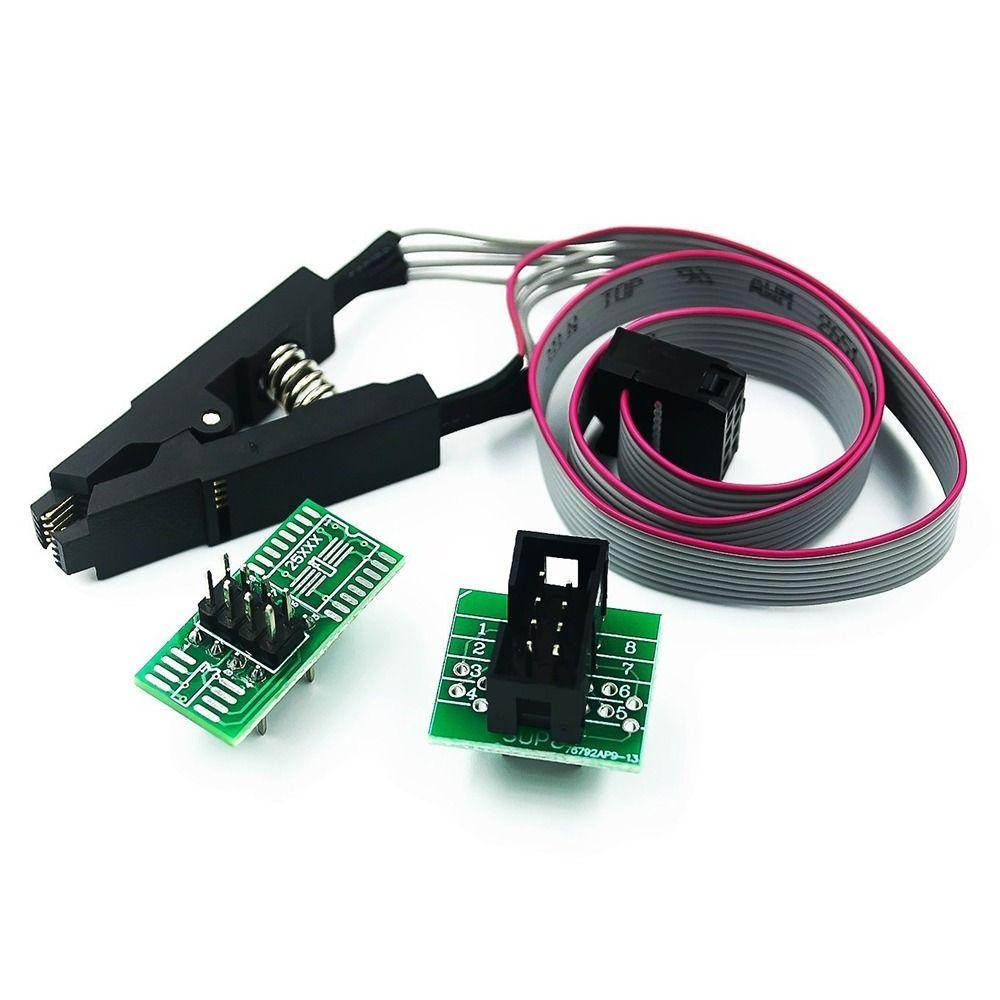
\includegraphics[width=0.4\textwidth]{images/device/programmer.jpeg}
    \caption{Programador \est{SOC8} amb pinça.}
    \label{fig:programmer}
\end{figure}

Per a programar per \acro{isp} s'ha utilitzat una placa Arduino amb el codi
\est{ArduinoISP}, disponible a la pròpia aplicació \est{ArduinoIDE}
\cite{ArduinoIsp}. Un cop
l'Arduino tenia aquest codi, una simple comanda d'\est{avrdude} s'ha afegit
al \est{Makefile}, permetent la programació senzilla del dispositiu.

\section{Actualitzacions de firmware}

Quan incrustar el programa no és una tasca trivial, cal preguntar-se què
passaria si  es vol actualitzar la versió del \est{firmware} per a afegir
funcionalitats o corregir errors. Queda clar que els consumidors no disposaran
de l'enginy de la figura \ref{fig:programmer}, ni dels coneixements necessaris
per a poder-lo utilitzar, pel que s'ha de tenir present alguna forma per a
poder canviar el codi del microcontrolador.

Una de les solucions més senzilles és tornar a posar el \est{Bootloader} a la
placa. D'aquesta forma, es podrà programar mitjançant la mateixa connexió
\acro{usb}, com s'ha fet durant l'etapa de desenvolupament. L'únic inconvenient
d'aquest sistema és que el dispositiu tardarà més a funcionar «amb normalitat»,
degut al temps que tarda en executar-se aquest codi inicial.

Una altra solució, però no aplicable per al \est{hardware} creat en aquest
projecte, és afegir un botó a la \acro{pcb} que, si es prem més de 3 segons,
atura el programa principal del dispositiu i inicia un programa que
fa la mateixa tasca que el \est{Bootloader}. Aquest botó també podria aportar
altres beneficis com, per exemple, configurar més fàcilment el dispositiu.

Finalment s'ha decidit no incorporar cap \est{Bootloader} en aquesta primera
tirada de dispositius, degut a la no imminent comercialització. Tot i això, s'ha
pres nota de la importància d'aquest aspecte per a tenir-lo present per a
futures versions de la placa de circuit imprès.
